\subsection{Stabilitätsbedingung des doppeltsphärischen Aufbaus}
Die Messdaten zur Stabilitätsbedingung des doppeltsphärischen Aufbaus sind in Tabelle \ref{tab:stabsphere} notiert.
\begin{table}[h!]
  \centering
  \caption{Messdaten zu Überprüfung der Stabilitätsbedingung des doppelspärischen Aufbaus}
  \label{tab:stabsphere}
  \begin{tabular}{c c c c}
    \toprule
%    \multicolumn{3}{c}{$f_{\text{1& theo}}=\SI{0,1}{m}$} & \multicolumn{3}{c}{$f_{\text{2& theo}}=\SI{0,05}{m}$}\\
      L/m & I/mA & L/m & I/mA \\
      \midrule
      0,59  & 0,50464 & 0,99  & 0,40644 \\
      0,63  & 0,46055 & 1,03  & 0,32881 \\
      0,67  & 0,46578 & 1,07  & 0,27833 \\
      0,71  & 0,46251 & 1,11  & 0,26431 \\
      0,75  & 0,54064 & 1,15  & 0,23698 \\
      0,79  & 0,53707 & 1,19  & 0,24564 \\
      0,83  & 0,56027 & 1,23  & 0,016685\\
      0,87  & 0,53085 & 1,27  & 0,22631 \\
      0,91  & 0,44278 & 1,31  & 0,21110 \\
      0,95  & 0,42519 & 1,35  & 0,29335 \\
    \bottomrule
  \end{tabular}
\end{table}

%\end{landscape}
%\end{document}

Die Resonatorlänge $L$ ist in Abbildung \ref{fig:stabsphere} gegen den aufgenommenen Strom $I$ des Photodetektors aufgetragen.
\begin{figure}
  \centering
  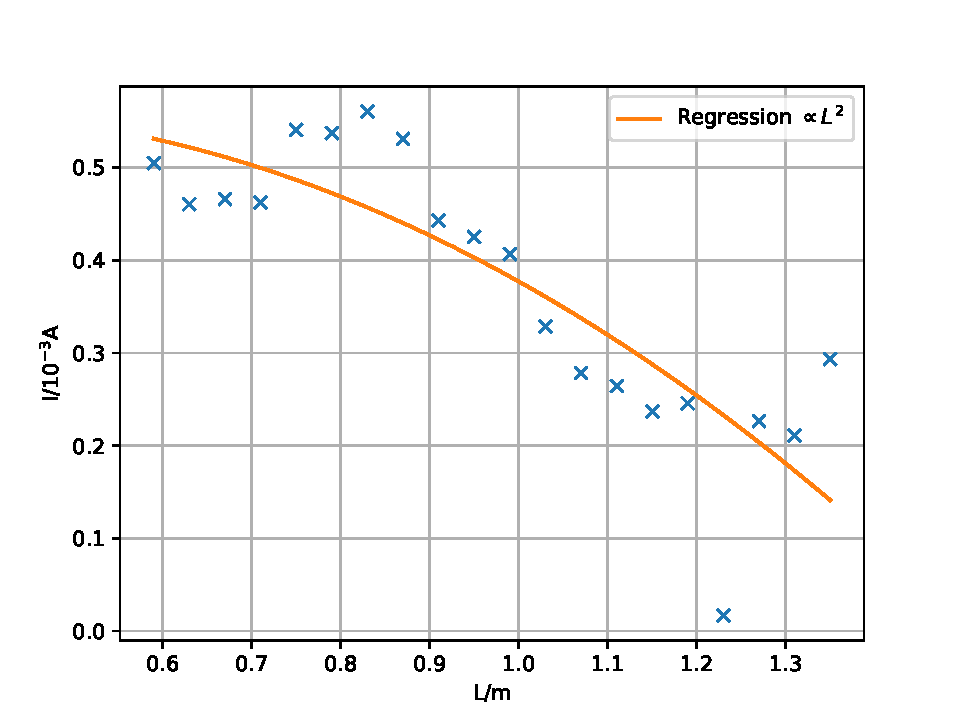
\includegraphics[width=\textwidth]{stabsphere.pdf}
  \caption{Überprüfung der Stabilitätsbedingung beim doppeltsphärischen Aufbau}
  \label{fig:stabsphere}
\end{figure}
Es wird folgende Funktion mit Python 3.6.3 (scipy.optimize, curve$\_$fit) gefittet:
\begin{equation*}
  I= \frac{a(L+b)^2}{r_1 r_2}+\frac{c(L+d)}{r_1 r_2}+\frac{e}{r_1 r_2}.
\end{equation*}
Es ergeben sich die Parameter
\begin{align*}
a &=& \SI{0.77019576  \pm 6.67239536e-01}{} \\
b &=& \SI{0.68148470  \pm 5.70376283e+12}{} \\
c &=& \SI{-1.53874317 \pm 1.35339234e+13}{} \\
d &=& \SI{2.97459567  \pm 1.52142773e+13}{} \\
e &=& \SI{3.19916773  \pm 1.03956309e+12}{}. \\
\end{align*}
\FloatBarrier

\subsection{Stabilitätsbedingung des sphärisch-flachen Aufbaus}
Die Messwerte zum Photodetektorstrom $I$ und der Resonatorlänge $L$ sind in Tabelle \ref{tab:stabflat} aufgenommen.
Aufgrund einer technischen Gegebenheit wird die Messung doppelt durchgeführt.
\begin{table}[h!]
  \centering
  \caption{Messdaten zu Überprüfung der Stabilitätsbedingung des sphärisch-flachen Aufbaus}
  \label{tab:stabflat}
  \begin{tabular}{c c c c}
    \toprule
    \multicolumn{2}{c}{Erste Messung} & \multicolumn{2}{c}{Zweite Messung}\\
      L/m & I/$\mu$A & L/m & I/$\mu$A \\
      \midrule
      0,57 & 5,0286  & 0,55 & 62,856 \\
      0,59 & 3,6969  & 0,57 & 62,001 \\
      0,63 & 10,6174 & 0,59 & 44,406 \\
      0,67 & 1,9912  & 0,61 & 45,883 \\
      0,71 & 0,38304 & 0,63 & 67,950 \\
      0,75 & 2,2791  & 0,65 & 50,739 \\
      0,79 & 5,5241  & 0,67 & 37,018 \\
      0,83 & 6,1024  & 0,69 & 13,102 \\
          &          & 0,71 & 25,690 \\
          &          & 0,73 & 15,603 \\
          &          & 0,75 & 15,836 \\
    \bottomrule
  \end{tabular}
\end{table}

%\end{landscape}
%\end{document}

In Abbildung \ref{fig:stabflat} ist der Photodetektorstrom $I$ in Abhängigkeit der Resonatorlänge $L$ dargestellt.
\begin{figure}
  \centering
  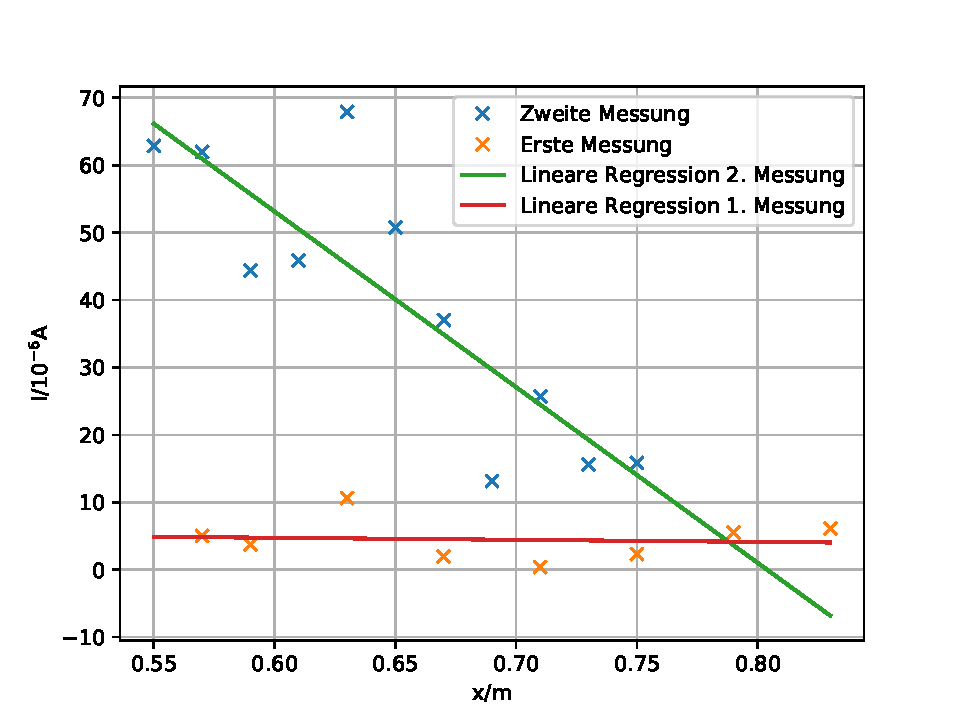
\includegraphics[width=\textwidth]{stabflat.pdf}
  \caption{Überprüfung der Stabilitätsbedingung beim sphärisch-flachen Aufbau}
  \label{fig:stabflat}
\end{figure}
Die lineare Regression hat die Form
\begin{equation*}
  I= aL+b
\end{equation*}
und wird erneut mit Python 3.6.3 (scipy.optimize, curve$\_$fit) durchgeführt.
Als Parameter ergeben sich:
\begin{align*}
&&\text{zweite Messung} \\
a &=& \SI{260.60636539 \pm 2739.59243164}{} \\
b &=& \SI{-209.49268296 \pm 1168.43618691}{} \\
&&\text{erste Messung} \\
a &=& \SI{3.03299421 \pm 187.11756018}{} \\
b &=& \SI{-6.55319099 \pm 91.18238783}{} \\
\end{align*}
\FloatBarrier

\subsection{Grundmode}
In Tabelle \ref{tab:grundmode} sind die Messwerte zur Intensitätsverteilung notiert.
\begin{table}[h!]
  \centering
  \caption{Messdaten zu Untersuchung der Grundmode}
  \label{tab:grundmode}
  \begin{tabular}{c c c c}
    \toprule
%    \multicolumn{2}{c}{Erste Messung} & \multicolumn{2}{c}{Zweite Messung}\\
      L/m & I/$\mu$A & L/m & I/$\mu$A \\
      \midrule
       0,031  &  0,01837  &  -0,003  &  1,68402 \\
       0,025  &  0,01850  &  -0,006  &  1,42631 \\
       0,020  &  0,03517  &  -0,009  &  1,00125 \\
       0,015  &  0,09141  &  -0,012  &  0,55967 \\
       0,012  &  0,22460  &  -0,015  &  0,24617 \\
       0,009  &  0,53102  &  -0,020  &  0,05179 \\
       0,006  &  0,97390  &  -0,025  &  0,02391 \\
       0,003  &  1,38290  &  -0,031  &  0,01991 \\
       0,000  &  1,63817  &    & \\
    \bottomrule
  \end{tabular}
\end{table}

%\end{landscape}
%\end{document}


\begin{figure}
  \centering
  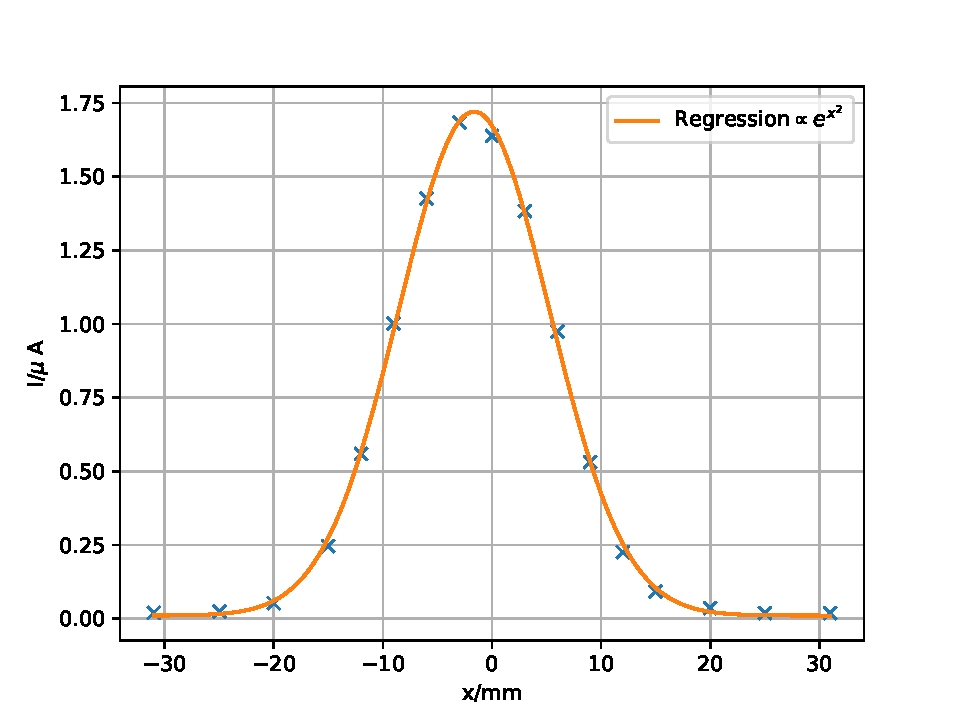
\includegraphics[width=\textwidth]{grundmode.pdf}
  \caption{Intensitätsverteilung der Grundmode}
  \label{fig:grundmode}
\end{figure}
Fit:
\begin{equation*}
  I= a \exp{\left( b(x-c)^2 \right)}+d
\end{equation*}
\begin{align*}
a &=& \SI{ 1.71042307 \pm 2.01428259e-04}{}\\
b &=& \SI{-0.01047146 \pm 5.10717911e-08}{}\\
c &=& \SI{-1.64149566 \pm 3.45206452e-03}{}\\
d &=& \SI{ 0.01007865 \pm 7.33843461e-05}{}\\
\end{align*}
\FloatBarrier

Erste Mode:
\begin{table}[h!]
  \centering
  \caption{Messdaten zu Untersuchung der ersten Mode}
  \label{tab:erstemode}
  \begin{tabular}{c c c c c c c c c c c c c c c c c}
    \toprule
%    \multicolumn{2}{c}{Erste Messung} & \multicolumn{2}{c}{Zweite Messung}\\
      L/m & I/nA & L/m & I/nA & L/m & I/nA & L/m & I/nA \\
      \midrule
       0,031  &  0,62978 & 0,014  &  18,897  &  0,000   &  3,566  & -0,014  &  13,895  \\
       0,029  &  0,48938 & 0,013  &  20,22   &  -0,001  &  1,637  & -0,015  &  10,420  \\
       0,027  &  2,24440 & 0,012  &  24,974  &  -0,002  &  1,031  & -0,016  &  8,870   \\
       0,025  &  0,92853 & 0,011  &  28,676  &  -0,003  &  2,950  & -0,017  &  6,652   \\
       0,023  &  2,68534 & 0,010  &  35,051  &  -0,004  &  6,667  & -0,018  &  3,354   \\
       0,022  &  5,0257  & 0,009  &  39,979  &  -0,005  &  11,173 & -0,019  &  2,127   \\
       0,021  &  6,2573  & 0,008  &  43,685  &  -0,006  &  16,513 & -0,020  &  1,442   \\
       0,020  &  5,2613  & 0,007  &  44,221  &  -0,007  &  20,980 & -0,021  &  0,673   \\
       0,019  &  3,6343  & 0,006  &  40,383  &  -0,008  &  23,424 & -0,022  &  0,441   \\
       0,018  &  4,0211  & 0,005  &  34,308  &  -0,009  &  27,747 & -0,023  &  0,426   \\
       0,018  &  1,1202  & 0,004  &  24,899  &  -0,010  &  26,445 & -0,025  &  0,501   \\
       0,017  &  8,8913  & 0,003  &  18,409  &  -0,011  &  24,102 & -0,027  &  0,431   \\
       0,016  &  14,7981 & 0,002  &  12,210  &  -0,012  &  21,381 & -0,029  &  0,621   \\
       0,015  &  18,0773 & 0,001  &  7,091   &  -0,013  &  17,631 & -0,031  &  0,859   \\

    \bottomrule
  \end{tabular}
\end{table}

%\end{landscape}
%\end{document}

\begin{align*}
kommt noch\\
\end{align*}
\FloatBarrier
